
% ---- fig001_iraz.pgf ----
% (c) 2013 Claudio Carboncini - claudio.carboncini@gmail.com
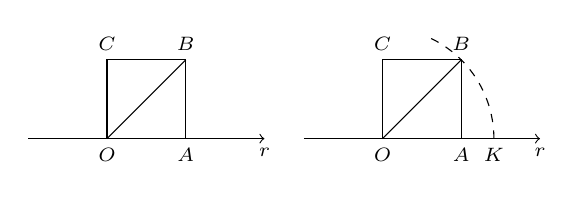
\begin{tikzpicture}[x=10mm, y=10mm, font=\scriptsize]
  \draw [->] (0,0) -- (3,0) node [below] () {$r$};
  \draw (1,0) rectangle (2,1);
  \draw (1,0) -- (2,1);

  \coordinate[label=below:$O$] (O) at (1,0);
  \coordinate[label=below:$A$] (A) at (2,0);
  \coordinate[label=above:$C$] (C) at (1,1);
  \coordinate[label=above:$B$] (B) at (2,1);

  \begin{scope}[xshift=35mm]
    \draw [->] (0,0) -- (3,0) node [below] () {$r$};
    \draw (1,0) rectangle (2,1);
    \draw (1,0) -- (2,1);

    \coordinate[label=below:$O$] (O) at (1,0);
    \coordinate[label=below:$A$] (A) at (2,0);
    \coordinate[label=above:$C$] (C) at (1,1);
    \coordinate[label=above:$B$] (B) at (2,1);
    \coordinate[label=below:$K$] (K) at (2.414,0);

    \draw[dashed] (2.414,0) arc [start angle=0, end angle=65,radius=1.414cm,];

  \end{scope}
\end{tikzpicture}
% -----------------

% ---- fig001_is.pgf ----
% (c) 2013 Claudio Carboncini - claudio.carboncini@gmail.com
\begin{tikzpicture}[font=\small,x=10mm, y=10mm]

\draw[->] (0,0) -- (8,0) node [below right] () {$r$};

\foreach \x in {2,5}{
\draw(\x,3pt)--(\x,-3pt);
\begin{scope}[dotted]
\draw (\x,0) -- (\x,-1.5);
\draw (0,-.5) -- (2,-.5);
\draw (0,-1) -- (5,-1);
\end{scope}}

\node[above]  at (2,0) {$-1$};
\node[above]  at (5,0) {$0$};
\pattern[pattern= north east lines, pattern color=red] (5,-1) rectangle (8,-1.5);

\node[below] () at (6.5,-1.5) {$\IS$};

\begin{scope}[blue,thick]
\draw (2,-.5) -- (8,-.5);
\draw (5,-1) -- (8,-1);

\draw[fill=blue] (2,-.5)circle (1.5pt);
\draw[fill=blue] (5,-1)circle (1.5pt);

\end{scope}

\end{tikzpicture}
% -----------------

% ---- fig002_seg.pgf ----
% (c) 2013 Claudio Carboncini - claudio.carboncini@gmail.com
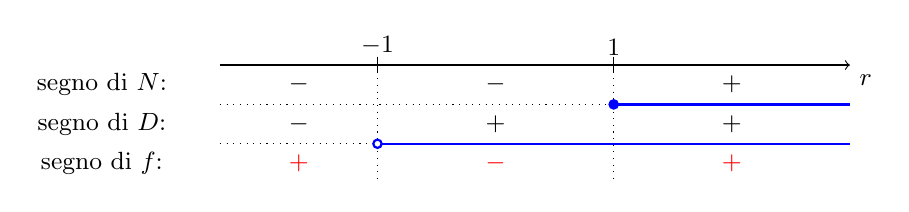
\begin{tikzpicture}[font=\small,x=10mm, y=10mm]

\draw[->] (0,0) -- (8,0) node [below right] () {$r$};

\foreach \x in {2,5}{
\draw(\x,3pt)--(\x,-3pt);
\begin{scope}[dotted]
\draw (\x,0) -- (\x,-1.5);
\draw (0,-.5) -- (5,-.5);
\draw (0,-1) -- (2,-1);
\end{scope}}

\node[above]  at (2,0) {$-1$};
\node[above]  at (5,0) {$1$};

\begin{scope}[blue,thick]
\draw (5,-.5) -- (8,-.5);
\draw (2,-1) -- (8,-1);

\draw[fill=blue] (5,-.5)circle (1.5pt);
\draw[fill=white] (2,-1)circle (1.5pt);
\end{scope}

\foreach \x in {-1.5}{
\node  at (\x,-.25) {segno di $N$:};
\node  at (\x,-.75) {segno di $D$:};
\node  at (\x,-1.25) {segno di $f$:};
}
\foreach \z in {1,3.5}{
\node  at (\z,-.25) {$-$};
}
\foreach \zi in {3.5, 6.5}{
\node  at (\zi,-.75) {$+$};
}

\node  at (6.5,-.25) {$+$};
\node  at (1,-.75) {$-$};

\begin{scope}[red]
\foreach \zii in {1, 6.5}{
\node  at (\zii,-1.25) {$+$};
}
\node  at (3.5,-1.25) {$-$};
\end{scope}
\end{tikzpicture}
% -----------------

% ---- fig003_seg.pgf ----
% (c) 2013 Claudio Carboncini - claudio.carboncini@gmail.com
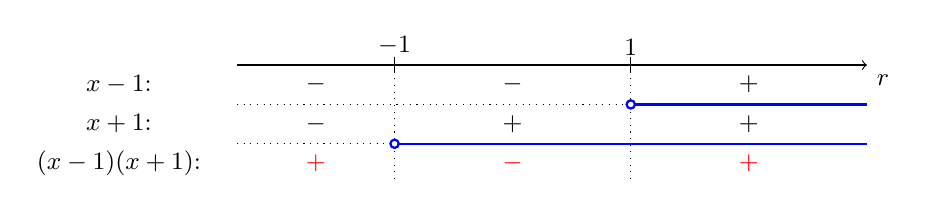
\begin{tikzpicture}[font=\small,x=10mm, y=10mm]

\draw[->] (0,0) -- (8,0) node [below right] () {$r$};

\foreach \x in {2,5}{
\draw(\x,3pt)--(\x,-3pt);
\begin{scope}[dotted]
\draw (\x,0) -- (\x,-1.5);
\draw (0,-.5) -- (5,-.5);
\draw (0,-1) -- (2,-1);
\end{scope}}

\node[above]  at (2,0) {$-1$};
\node[above]  at (5,0) {$1$};

\begin{scope}[blue,thick]
\draw (5,-.5) -- (8,-.5);
\draw (2,-1) -- (8,-1);

\draw[fill=white] (5,-.5)circle (1.5pt);
\draw[fill=white] (2,-1)circle (1.5pt);
\end{scope}

\foreach \x in {-1.5}{
\node  at (\x,-.25) {$x-1$:};
\node  at (\x,-.75) {$x+1$:};
\node  at (\x,-1.25) {$(x-1)(x+1)$:};
}
\foreach \z in {1,3.5}{
\node  at (\z,-.25) {$-$};
}
\foreach \zi in {3.5, 6.5}{
\node  at (\zi,-.75) {$+$};
}

\node  at (6.5,-.25) {$+$};
\node  at (1,-.75) {$-$};

\begin{scope}[red]
\foreach \zii in {1, 6.5}{
\node  at (\zii,-1.25) {$+$};
}
\node  at (3.5,-1.25) {$-$};
\end{scope}
\end{tikzpicture}
% -----------------
